\documentclass{jlreq}
\usepackage{float}
\usepackage{graphicx}

\title{人工生命と進化型計算}
\author{学籍番号: 02230471 氏名: 佐藤雅文}
\date{提出日: 2026年2月4日}

\begin{document}
\maketitle

\section {パーコレーション}
% イントロダクション
全体として、正方格子/三角格子のボンド/サイトパーコレーションのシミュレーション、また臨界確率に関する考察を行った。
\par
シミュレーションでは、パーコレーションモデルをUnion-Find法をベースに実装した。
Union-Find法とは、グループを木構造で管理する方法であり、
グループ同士を結合するUnionと要素が属するグループの根要素がどれかを探すFindの2つの操作からなる。
Findする際に、辿って通った要素全てを直接根要素に付け替えながら根要素を探すので、
木構造が浅くなり、親要素を辿る操作が非常に速いことに特徴がある。
\par
また、パーコレーションモデルでは、その最上辺の格子点にひとつでも水が流れていて、
かつ最下辺の格子点にひとつでも水が流れているかどうかを浸透の判定基準とし、
開いている点または辺を繋いでいく作業をUnion-Find法のUnionの操作に対応させ、
最上辺と最下辺がつながっているかどうかを判定する。
\par
なお、コード上では簡単のため、最上辺と最下辺をそれぞれ全て仮想の点VirtualTopとVirtualBottomにUnionし、
VirtualTopとVirtualBottomがUnionされているかを浸透の基準としている。
\par
シミュレーションコードはJavaで実装した。
その際のクラス図は以下の図のようである。

\begin{figure}
    \centering
    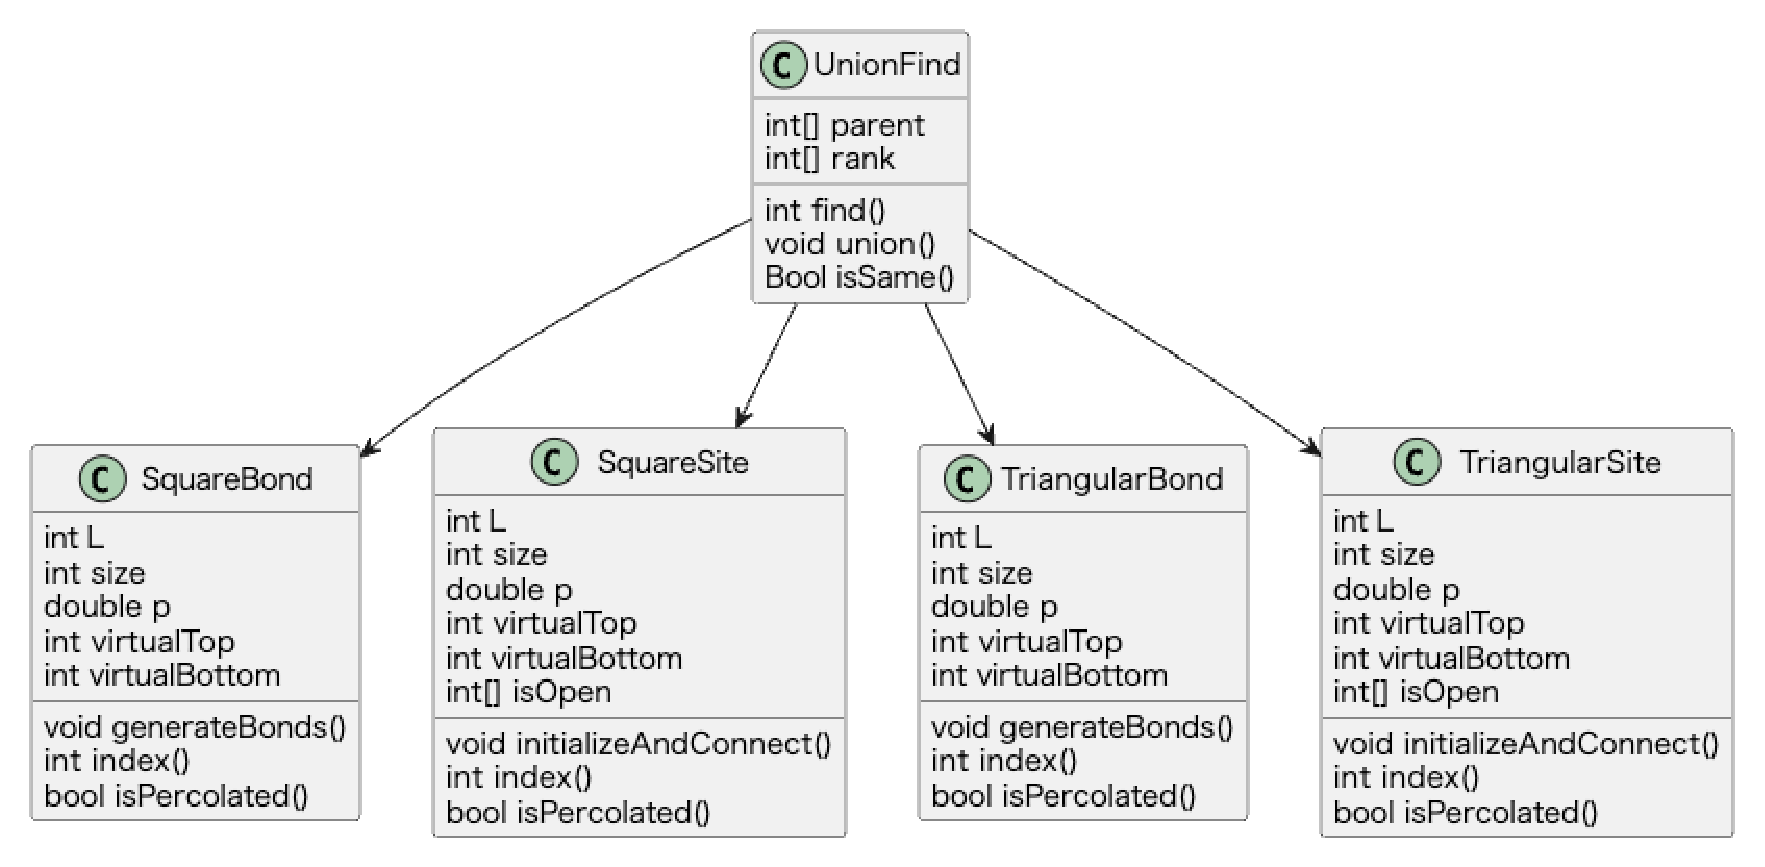
\includegraphics[width=0.8\linewidth]{percolationClassUML.eps}
    \caption{パーコレーションモデルクラス図}
\end{figure}




\subsection{正方格子ボンドパーコレーション}
\subsubsection{シミュレーション}


\subsection{正方格子サイトパーコレーション}

\subsection{三角格子ボンドパーコレーション}

\subsection{三角格子サイトパーコレーション}


\end{document}